

\subsection{Alkuperäinen ominaisuus ja parannus kohteet}
%selitys mykyisestä sivusta ja featuresta. ja mihin se pitää muokata


Sovelluksessa on "Progressio"{} niminen ominaisuus. 
Ominaisuus antaa mahdollisuuden määrittää käyttäjälle, jokin "mitattava"{} arvo.
Kuvassa \nextImageCount {} näkyy on progressio sivu, täältä käyttäjä voi merkata ja seurata kyseistä mitattavaa arvoa.

\bigskip


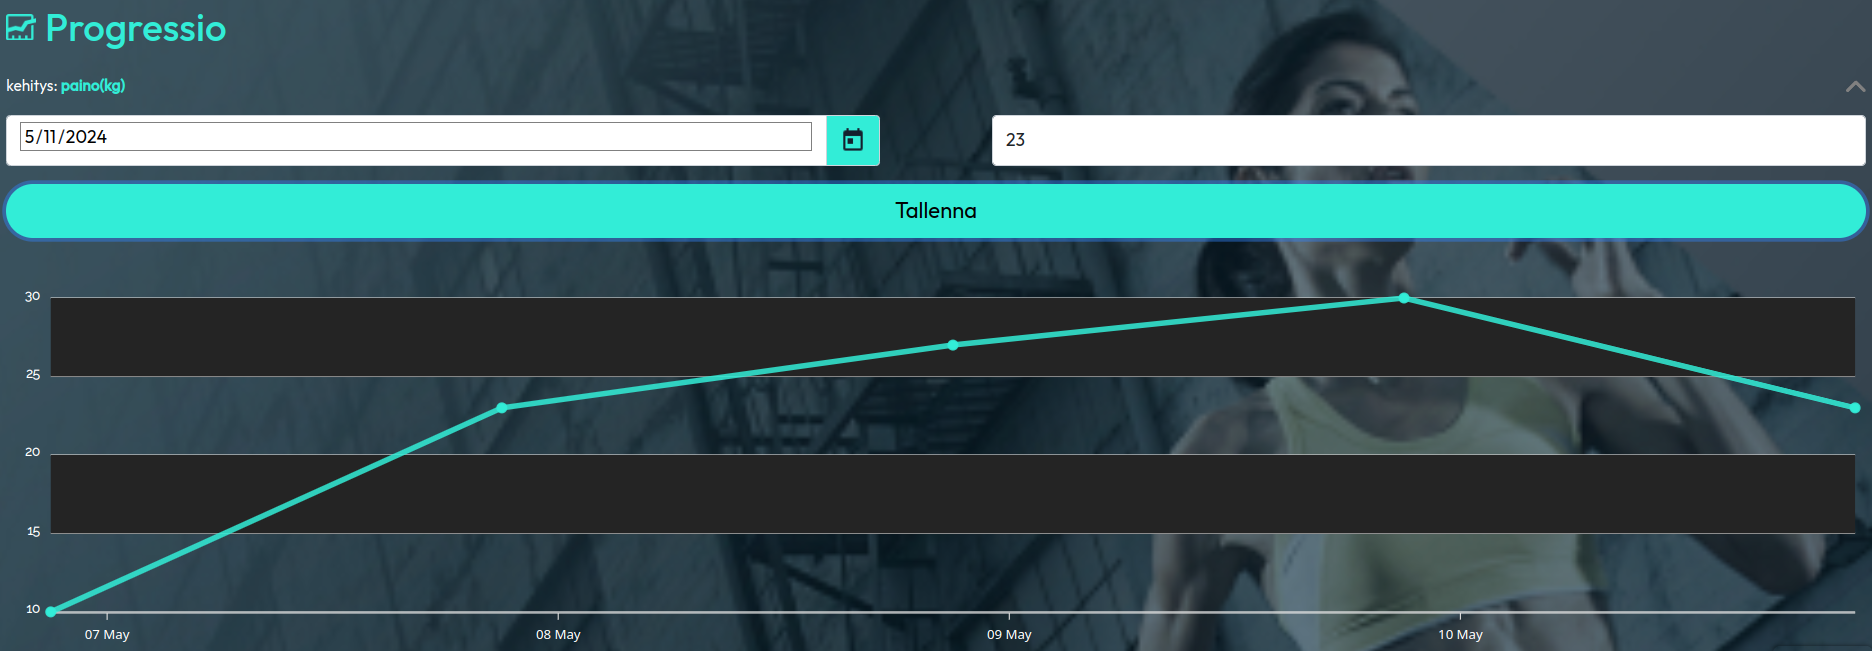
\includegraphics[width =15cm]{src/public/progressiosingle.png}\\
Kuva \getImgCount {}. Progressio sivu (tarvitsee paremman kuvan)
\medskip

Kuvassa \theimgCounter {} mitataan painoa kg:na. Käyttäjä pystyy valitsemaan miltä päivältä arvo on otettu ja mikä itse arvo on.
% asiakieli työnanataja haluaa
Työnanataja haluaa, että käyttäjälle voisi määritellä useamman mitattavan arvon ja, 
että Progressio sivulta käyttäjä pystyisi seuraamaan ja tallentamaan useampia eri mittausarvoja.
\medskip


Käyttäjän mitattavan arvon suure säilytetään käyttäjän profiilissa merkkijonona. 
Kuvassa \nextImageCount {} on esimerkki käyttäjä profiilin skeemasta JSON muodossa.
Yksittäinen "measurableThing"{} ominaisuus ei ole riittävä useamman mitattavan arvon seurantaan, joten se pitäisi vaihtaa.
%mainitse paremmin mongo nosql dokumentti
Koska käytössä on nosql dokumentti voimme vaihtaa "measurableThing"{} merkkijonon, "measurableThings"{} merkkijono listaan.
\bigskip



Kuva \getImgCount {}. Käyttäjä profiilin skeema
\medskip













\subsection{Ominaisuuden totetus}


\subsubsection{Käyttäjä profiili skeeman migraatio}

% tiukka skaama
MongoDB:n NoSql dokumentti ei määritä tiukkaa skeemaa joten käyttäjien skeemat voivat olla eriävät.
Skeeman muutos vaatii jokaisen käyttäjän profiilin muokkaamista haluttuun muotoon.
Käyttäjä profiilin skeeman muutos pitää tehdä kaikille aktiivisille käyttäjille, käyttäjän luonnissa pitää myös muokata siten, 
että uudet käyttäjän alkaisivat käyttämään uutta skeemaa.
%selitä paremmin
Projektissa on myös käytössä ominaisuus tarkastus rajapinnoissa ettei mongodb kantaan voida tallettaa tietoa jota sinne ei haluta.
%api muutos
\medskip

selitys migraatio prosessista. teoriaa migraatiosta myös.
migraatio tehdään migraatio kuvan \nextImageCount {} migraatio funktiolla. 
Funktio käy läpi kaikki käyttäjät jolla measurableThing ominaisuus on olemassa ja päivittää sen measurableThings listaan.
%mnnm
Projektissa on tarpeeksi vähän käyttäjiä, joten migraatio tehdään synkroonisesti palvelimella. 
Jos projektissa olisi isompi määrä käyttäjiä tämä operaatio pysäyttäisi palvelimen sen ajaksi kun käyttäjä profiileja päivitettäisiin.
Isoimmilla käyttäjä määrillä tämä operaatio tehtäisiin huolto aikana, jolloin sovellus ei olisi käytössä tai asynkroonisesti, 
jolloin käyttäjiä migraoitaisiin pikkuhiljaa.


\bigskip

kuva migraatio funktiosta
\medskip

\bigskip


kuva uudesta skeemasta
\medskip









\subsubsection{Käyttöliittymä}

Käyttöliittymää pitää muokata siten,
että käyttäjä voi vaihtaa mitä mitattavaa arvoa hän haluaa seurata tai mihin mitattavaan arvoon hän haluaa tallentaa lukemia.

Käyttöliittymä pitää muokata sopivaksi skeema muutoksien kanssa. 
%more words
\bigskip


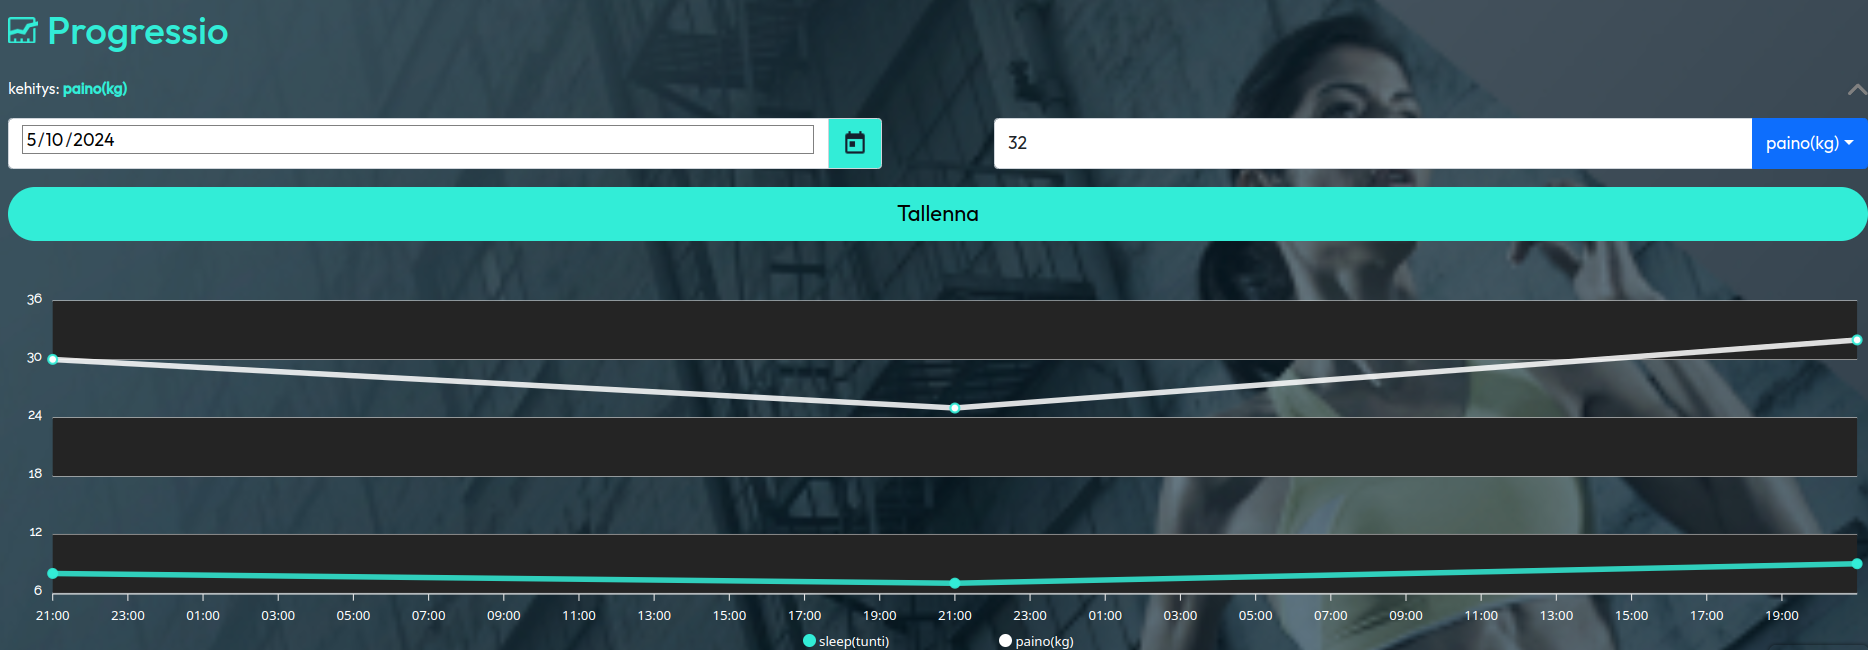
\includegraphics[width = 15cm]{src/public/progressmulti.png}\\
Kuva \getImgCount {}. Käyttäjän käyttöliittymä, muutoksien jälkeen 
\medskip

Käyttöliittymässä käyttäjällä on mahdollisuus valita mihin mitattavaan suurteeseen hän haluaa tallettaa arvoja kuvan \nextImageCount{} laskuvalikolla.
Kaavioon on lisätty uudet mitattavat arvot. 
%jotain kaaviosta ja siihen datan lisäämisestä
%more words
\bigskip

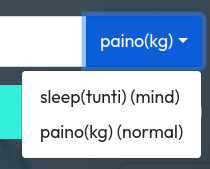
\includegraphics{src/public/progressselect.png}\\
Kuva \getImgCount {}. käyttöliittymän laskkuvalikosta
\medskip



Kuvassa \nextImageCount {} on päivitetty käyttäjän luomis käyttöliittymä.
Käyttöliittymään on lisätty nappi, josta voi lisätä, nimetä ja poistaa mitattavia suureita käyttäjälle.
%selitä paremmin että voi uudelleen käyttää komponenttia. tarviin jonkun sanan tolle yhdistelmälle
Tekstikenttä ja poisto nappi on sisällytetty React komponenttiin "MeasurableThingElement". 
Tämä antaa mahdollisuuden lisätä uusia kenttiä napista, tekemällä uuden instanssin komponentista.
%

\bigskip
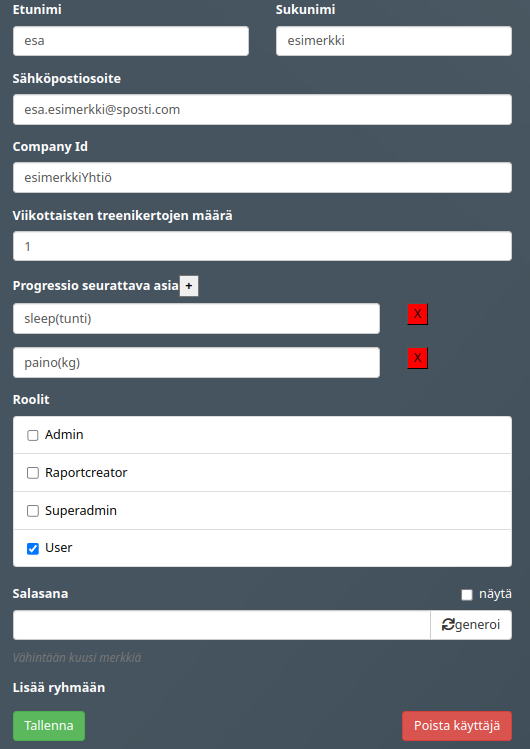
\includegraphics[width = 10cm]{src/public/oppar/adminUserProfilePost.png}\\
Kuva \getImgCount {}. käyttäjä luomis käyttöliittymä (cencor roles?)
\bigskip


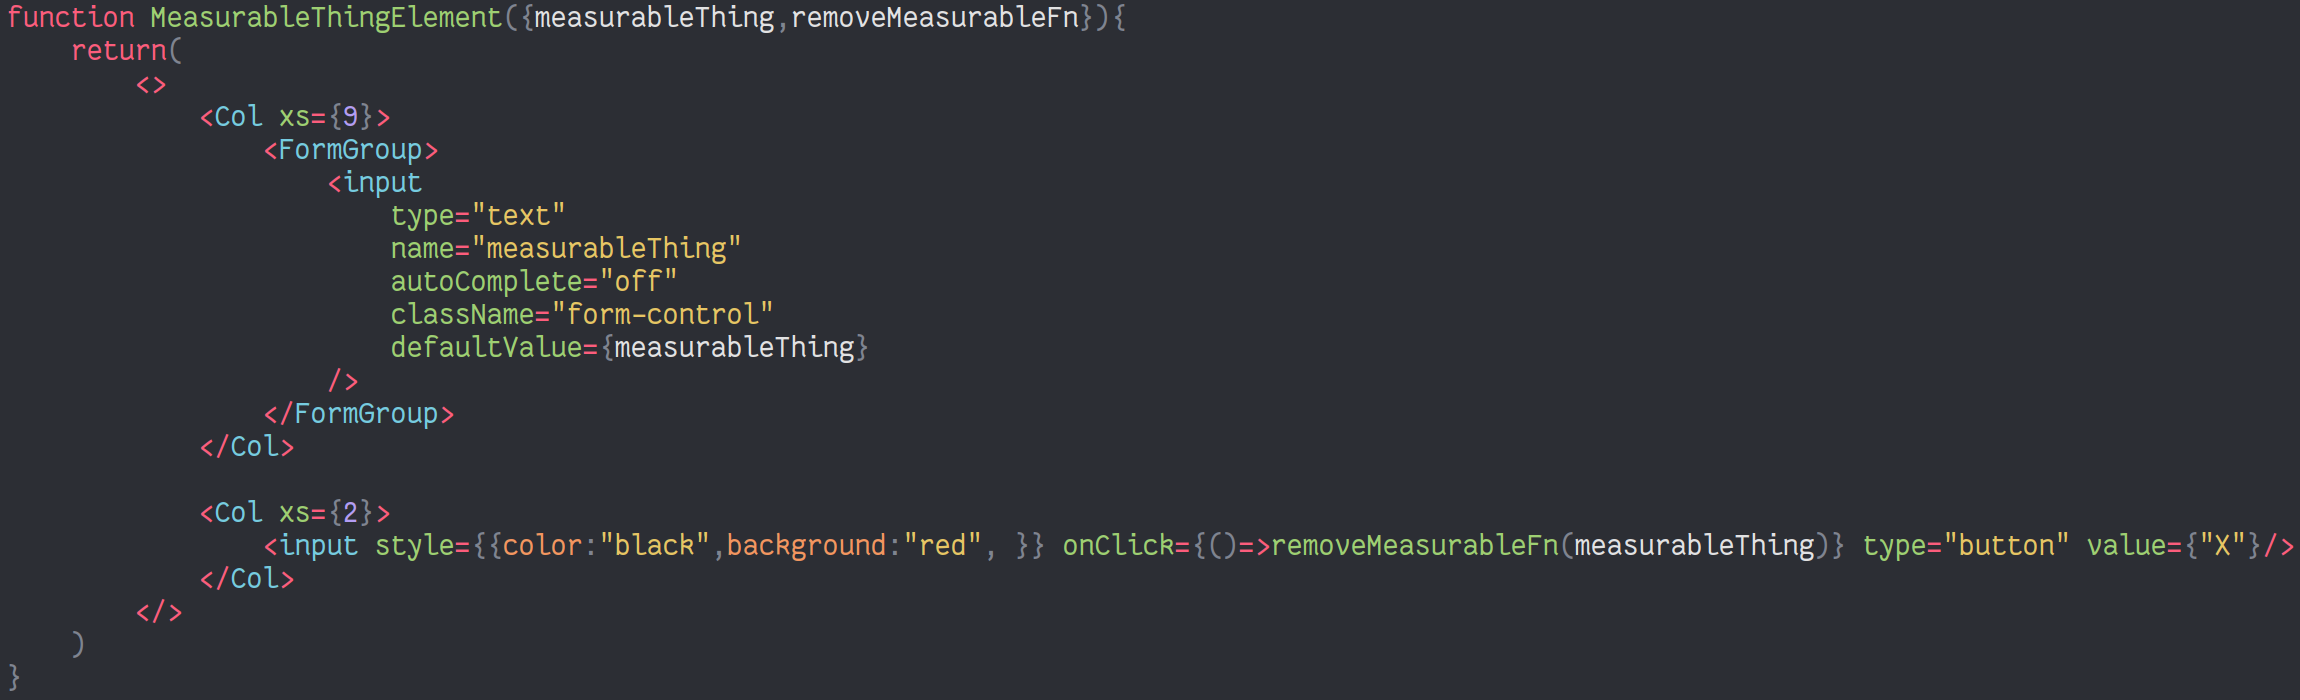
\includegraphics[width = 15cm]{src/public/oppar/measurableElementComponent.png}\\
Kuva \getImgCount {}. Mitattava elementti komponentti
\medskip

Komponentti on tilaton funktiokomponentti johon annetaan mitattavan suurteen nimi ja poista funktio proppeina.
Poinsto funktiota kutsutaan kun painetaan punaista X nappia ja se poistaa mitattavan suurteen käyttäjän profiilista ja elementin käyttöliittymästä.
%{\the\numexpr \theimgCounter + 2 }
\medskip


Entisessä käyttöliittymässä kuvassa \nextImageCount {} on vain yksi teksti kenttä, josta pystyi muuttamaan measurableThing ominaisuutta.
%toinen paragraafi
\bigskip


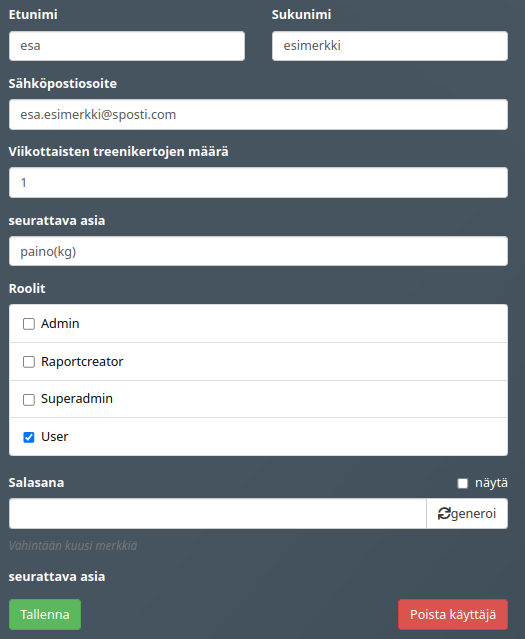
\includegraphics[width = 10cm]{src/public/oppar/adminUserProfilePre.png}\\
Kuva \getImgCount {}. Käyttäjän luomis käyttöliittymä ennen muutoksia (cencor roles?)
\medskip










\subsection{Ominaisuuden lopputulos ja käyttöönotto}


migrate meni hyvin. tosin jos olisi ottanut backupin databasesta niin ei olisi ollut riskiä hajottaa kaikkea.
\medskip

itse feature toimi hyvin käyttöön oton jälkeen ja kaikki käyttäjät saivat ominaisuuden käyttöön.
\medskip

käyttöliittymästän toiminnasta tai sen ulkonäöstä ei tullut palautetta sen jälkeen kun se oltiin käyttöön otettu joten sekin meni hyvin.
\medskip

